% Convolution appendix. 

\subsection{Introduction}

fMRI data presents a distinct challenge for relating neural stimuli 
to BOLD (blood-oxygen-level dependent) response. fMRI scans record changes 
in oxygenation levels of hemoglobin in the brain. However, there is a delay 
between the neural stimulus and the change in blood oxygen levels in a given 
area. In our case, the neural stimulation comes from a event-related style of 
experiment. A commonly assumed hemodynamic response to a neurological 
stimulation is the double gamma function that can be seen in Figure 
\ref{fig:hrf}. The complete hemodynamic response function needs to be modeled 
in order to better relate stimulation and the BOLD response from the fMRI scan.
It should be noted that the BOLD response is highly noisy and we're really 
trying to capture the blood oxygenation level change to the stimulation.

\subsection{Mathematics}
\subsubsection{Convolution Theory and Mathematics}

To relate stimuli to BOLD response, we convolved the time courses of discrete 
stimulation with the assumed response to a single stimulation.. At a basic 
level, convolution is a distinct combination of two functions (say $f$ and 
$g$). This combination is just the ``integral that expresses the amount of 
overlap of $f$ as it is shifted over another function $g$'' 
\cite{weissten2015convolution}. 
There are many examples of this, but the following is basic idea that we will 
expand off of later. 

Let us define the function $f$ as a sum of two gamma functions and $g$ as a 
``continuous'' specialized step function (we will examine why these functions 
are valuable later). Graphically, we can see their plots in Figure \ref{fig:f}
and \ref{fig:g}, and mathematically we will define them as in the following 
equations \ref{eq:gamma2} and \ref{eq:step}, respectively.

\begin{equation} \label{eq:gamma2}
f(t)=\frac{.6}{.17}\cdot  \big[G_1(6,t)-.35 \cdot G_1(12,t) \big]
\end{equation}

where $G_1(k,t) =\frac{1}{\Gamma(k)} t^{k-1} e^{-t}$ (the gamma pdf with 
$\theta =1$)

\begin{equation} \label{eq:step}
 g(t)=\Big \{ \begin{tabular}{l c}
 		0  & if  5.85 $\leq$ t $\leq$ 6.15\\
 		.6  & otherwise \\
 		\end{tabular} \end{equation}
 		
 		
\begin{figure}[ht]
\centering
\begin{minipage}[b]{0.45\linewidth}
	\centering
	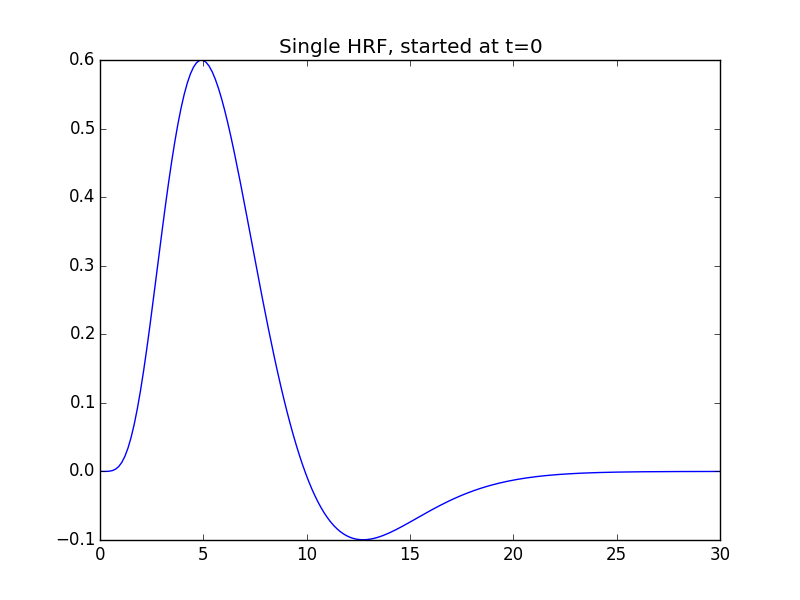
\includegraphics[width=.8\linewidth]{../images/hrf_pattern.png} 
	\caption{$f$ (``Stabilized Function'').}
	\label{fig:f}
\end{minipage}	
\quad
\begin{minipage}[b]{0.45\linewidth}
	\centering
		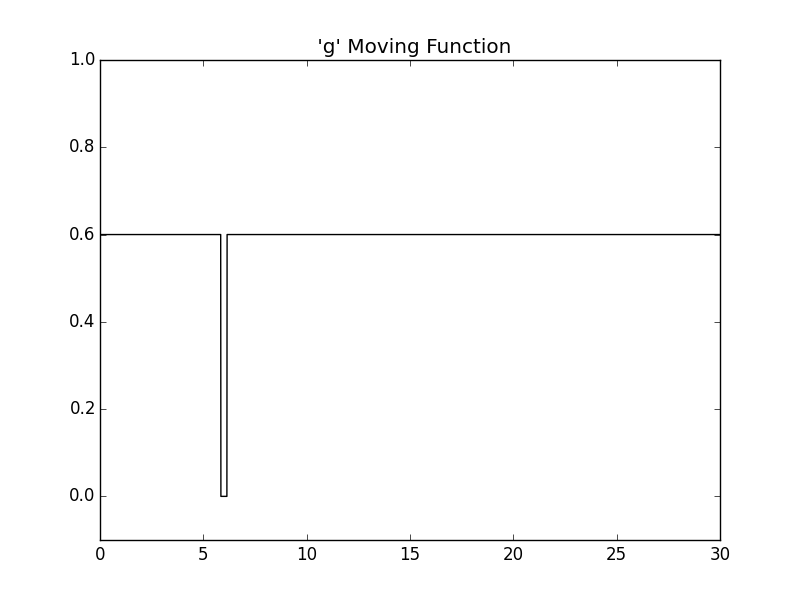
\includegraphics[width=.8\linewidth]{../images/play.png} 
	\caption{$g$ (``Moving function'').}
	\label{fig:g}
\end{minipage}
\end{figure}


As mentioned in the earlier definition, if we move $g$ across $f$ from 
left to right, we will see something similar to Figure \ref{fig:math} for 
discrete time intervals. If we plot these values (the integration of the 
differences), we will get a plot very similar to that of $f$ when $f$ is 
starting at a certain point. (The plot actually ``cheats'' when $f$ is 
negative, and we would have to alter definitions a little bit). If we had 
multiple peaks in our $g$ function (i.e. multiple distinct``zero'' places), we 
would expect to get multiple non-zero differences between the functions at 
each time capture. 

\begin{figure}[ht]
	\centering
	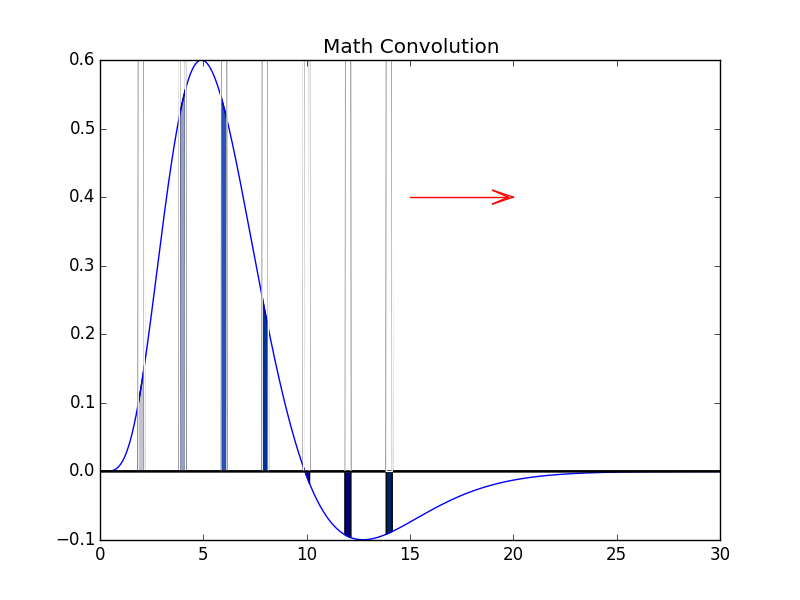
\includegraphics[width=.5\linewidth]{../images/math_convolved.png}
	\caption{Convolution of $f$ and $g$.}
	\label{fig:math}
\end{figure}


\subsubsection{Convolution Applied to Stimulus}

The ``continuous'' nature of the step function ``g'' does not extend well into 
the discrete time series that we have. However, one approach for fMRI analysis 
is to approach the convolution as something slightly different: mathematical 
sums. For example, in the previous section, we can treat $f$ as the same, and 
$g$ as $g'$ defined in equation \ref{eq:g_prime}.

\begin{equation}\label{eq:g_prime}
 g'(t)=\Big \{ \begin{tabular}{l c}
 		1  & if t=6\\
 		0  & otherwise \\
 		\end{tabular} \end{equation}

We could then find the value of the convolution of $g'$ and $f$ for discrete 
integers as in equation \ref{eq:math_discrete}.


\begin{equation}  \label{eq:math_discrete}
r(t)=  f(t-6)
\end{equation}



If we allow for multiple non-zero periods in $g'$, we can get a more general 
model in equation \ref{eq:math_discrete_extend}, where each $t_i$ is a value 
when $g'(t_i) \neq 0$: 

\begin{equation}  \label{eq:math_discrete_extend}
r(t)= \sum_{i=1}^n f(t-t_i)
\end{equation}

This equation gives a good glimpse into what the hemodynamic response would be 
after stimulus at time $t_i$ for $i \in {1,...,n}$. Moreover, one could extend 
the idea to include a ``strength'' value of the stimulus by changing the 
$g'(t_i)$ to values other than 1. If that was the case, we would change 
the response equation to Equation \ref{eq:math_discrete_final} to allow us to 
include all discrete $t$ into the equation where $g'(t_i)$ is now expected to 
be zero (so $n$ becomes much larger). 

\begin{equation}  \label{eq:math_discrete_final}
r(t)= \sum_{i=1}^n g'(t_i) f(t-t_i)
\end{equation}


With this new equation, we can consider function $f$ and $g'$ displayed 
graphically [Figure \ref{fig:hrf}, \ref{fig:on_off}, respectively] and 
their ``convolved'' output [Figure \ref{fig:convolve1}].




\begin{figure}[ht]
\centering
\begin{minipage}[b]{0.45\linewidth}
	\centering
	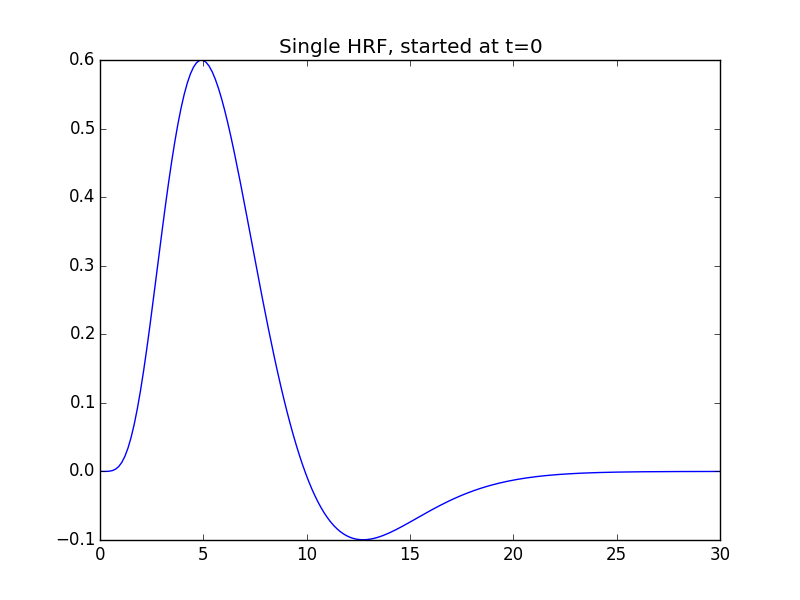
\includegraphics[width=.8\linewidth]{../images/hrf_pattern.png} 
	\caption{$f$ (``Stabilized Function'').}
	\label{fig:hrf}
\end{minipage}	
\quad
\begin{minipage}[b]{0.45\linewidth}
	\centering
	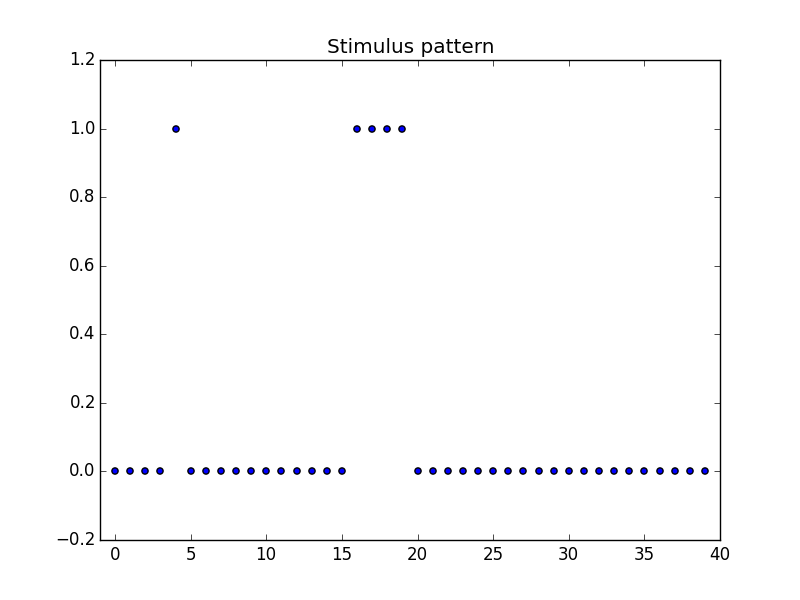
\includegraphics[width=.8\linewidth]{../images/on_off_pattern.png} 
	\caption{$g'$ (``Moving function'').}
	\label{fig:on_off}
\end{minipage}
\end{figure}


\begin{figure}[ht]
	\centering
	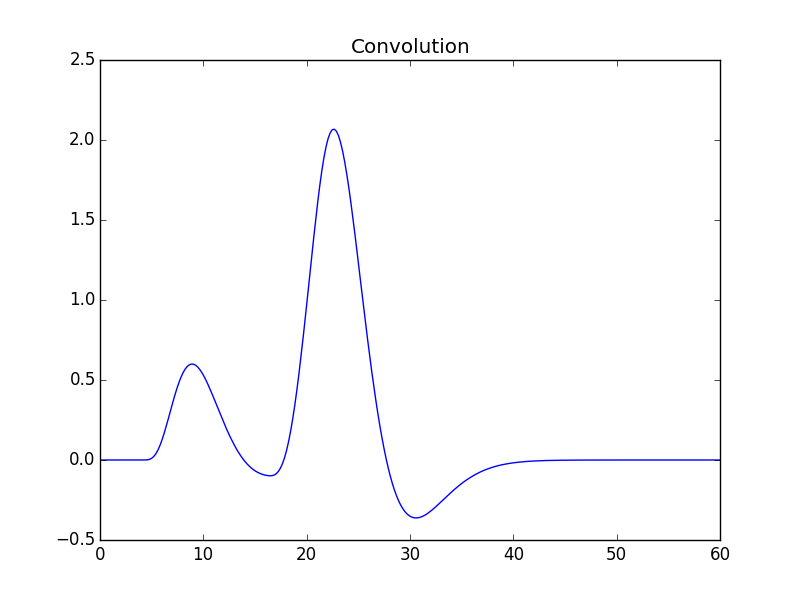
\includegraphics[width=.5\linewidth]{../images/initial_convolved.png}
	\caption{Convolution of $f$ and $g'$.}
	\label{fig:convolve1}
\end{figure}

\subsection{Approach to our Specific Problem}

\subsubsection{Returning to Our fMRI Data}

We can now apply this discrete approach to convolution between $f$ and $g'$ 
to our data. The $f$ is actually a common representation of the hemodynamic 
response, and the $g'$ is a good representation of the stimuli from an 
event-related trial \cite{brett2015course}. 

\subsubsection{Naive Approach (using \texttt{np.convolve})}

A \texttt{numpy} function \texttt{np.convolve}, which takes advantage of 
fast Fourier transforms for efficiency (it boils down to fewer computations 
using roots of unity) is commonly used to do discrete convolution. A naive 
approach for convolving two functions would use this function directly, but
\texttt{np.convolve} assumes that the intervals between stimuli mirror the 
desired intervals between prediction intervals. As such, we can not naively
apply the \texttt{np.convolve} for our data (though we do for a base model). 
Even still, exploring this naive approach to convolve the hemodynamic response 
gives an idea about what not to do, and sets a higher bar for efficiency.

\subsubsection{Needed Improvements: Moving beyond naive \texttt{np.convolve}}

Our data fails to meet the assumption that the intervals are in equidistant 
which was required to naively apply \texttt{np.convolve}. Especially in our 
case, there was not an simple fix, such as performing some basic rounding in 
order to then correctly utilize \texttt{np.convolve}. All the following 
approaches improve onthe basic \texttt{np.convolve} approach's accuracy, but 
ultimately circle back to incorporating \texttt{np.convolve} to improve the 
speed of the convolution.

Our condition file (\texttt{cond1}) lists stimulus times for when the 
individual pumped the balloon but did not pop it. For subject 001, the 
first 10 data points are as follows [Figure \ref{table:cond1}]:

\vspace{5mm}

\begin{figure}[ht]
\begin{center}
\begin{tabular}{|cccccccccc|}
  \hline
0.0671 &
2.1251 &
3.7681 &
5.6601 &
7.8673 &
9.3443 &
19.7831 &
22.0402 &
23.5837 &
25.1434 \\
 \hline

  \end{tabular}
   \caption{First 10 values for Sub 001, condition 1.}
  \label{table:cond1}
\end{center}
\end{figure}
 
Clearly, this short time series does not align with idealized scans that 
start at $t=0$ and occur every two seconds apart. As such, we had to go back 
to the drawing board to try to reproduce our expected hemodynamic response for 
the entire time course.


\subsection{Summary of Approaches}
Our first approach attempts to correctly match the theory underlying our data. 
Our second approach tries to utilize \texttt{np.convolve} by expanding the 
grid of desired results (thanks to advice from  Matthew Brett, Jean-Baptiste 
Poline, and Jarrod Millman).


\subsubsection{Initial Correction to Represent Theoretical Idea}
To account for our data's lack of any easily identifiable grid structure 
between when a stimulus was recorded and when our scans occurred (on the 
order of every 2 seconds), we went back to the theory of convolution and 
implemented code to recreate equation \ref{eq:math_discrete_final} directly. 
To do so, we also had to create a function that works with all discrete points 
of $f$, the stimulus response as potential starts of the hemodyamic response, 
multiplied by the actual value of $f$, as seen in equation 
\ref{eq:code_convolve}:

\begin{equation} \label{eq:code_convolve}
r(t)= \sum_{i=1}^n g'_{i} f(t-t_i)
\end{equation}

where $g'_{i}$ is the value of $g'$ at $t_i$ (allowing for zeros and varying 
non-zero values of $g'$).


\subsubsection{Matrix Multiplication}
Equation \ref{eq:code_convolve}, reproduced below

$$r(t)= \sum_{i=1}^n g'_{i} f(t-t_i)$$

can be rewritten as a matrix multiplication problem (thanks to Jane Liang), 
and can be seen below:

\begin{equation} \label{eq:matrix_code_convolve}
r(t)=  g^*(t)^T f^*(t)
\end{equation}

where $g^*$ is a vectorized function of $g'$ of $t$ as a scalar output and 
$f^*$ is the vector of $f$ values (irrespective of location, as the $t^*$ 
takes that into account). This is a useful representation, since matrix 
multiplication is faster for Python's numpy arrays. 


\subsubsection{Using FFT with \texttt{np.convolve}}
The ``theoretical'' solution lacked computation efficiency (despite 
considerable speed improvements from matrix multiplication), so we also 
approached the problem by creating a denser grid between each scan (two seconds 
apart). Then we rounded the actual times of the stimulus to meet this more 
finely scaled grid. This allowed us to utilize \texttt{np.convolve} with its 
faster algorithms (thanks to FFT), before reducing back down to our two second 
grid. 


\subsection{Example}

Now that we have discussed the theoretics of and possible implementations of 
the convolving event-related stimulation, let's look at a basic example from 
our data.(specifically using subject 001 condition files). In doing so, we 
examine the trade-offs between theoretical accuracy and computational 
efficiency.


\begin{figure}[ht]
\centering
	\begin{minipage}[b]{0.45\linewidth}
		\centering
		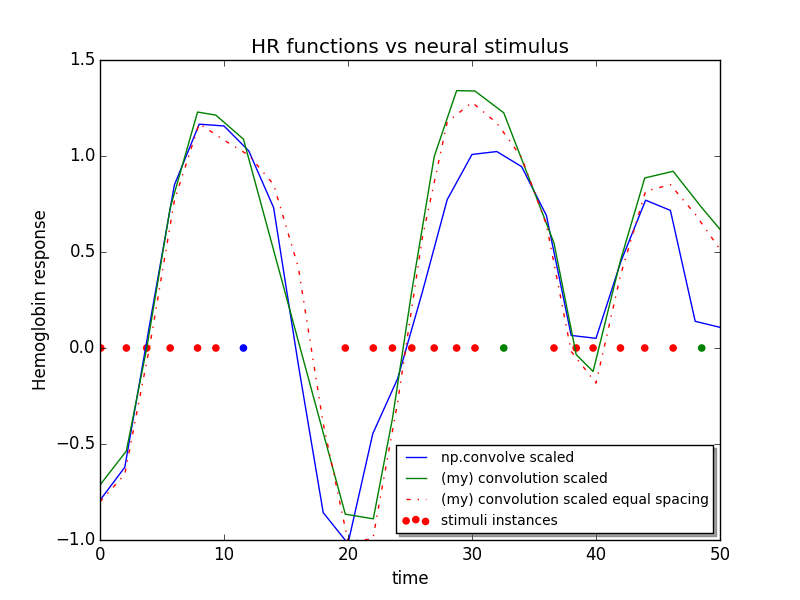
\includegraphics[width=.8\linewidth]{../images/convolution_vs_neural_stimulus}
		% needs to be from the event_related_HRF_script2.py 
		\caption{\scriptsize{Different convolution functions vs. the Neural stimulus}}
		\label{fig:convolution}

	\end{minipage}
\quad
	\begin{minipage}[b]{0.45\linewidth}
		\centering
		\begin{tabular}{|l | c|}
		\hline
		name in graph       & Speed per loop \\
		\hline
		np naive approach & 14.4 $\mu$s  \\
		user 2     		    & 972 ms  \\
		user 3     		    & 1.15 s    \\
		user 4 (15 cuts)      & 98.3 ms \\
		user 4 (30 cuts)      & 185 ms  \\
		user 5     	 	    & 110 ms   \\
		\hline
		\end{tabular}
		\vspace{5mm}
		\caption{\scriptsize{Speed to create HRF predictions for Subject 001, 
		all conditions}}
		\label{table:convolution}
	\end{minipage}
\end{figure}

The first method in the table ``np naive approach'' method blindly plugs 
in our data into the \texttt{np.convolve} function, provided to showcase 
potential speed. The ``user 2'' method  was the first approach to match the 
theory, though it matches the stimulation times instead of the scan times. 
The ``user 3'' method is the most theoretically sound model (and is our 
standard for accuracy). ``User 5'' model  is our matrix version of the theory, 
and has the same accuracy as ``user 3'', but is observably faster. The 
``user 4'' models fall under use the grid cut usage of \texttt{np.convolve}
with notations for the number of slices between each scan. We concluded that 
"user 4 (15 cuts)" was the best approach since it gives us speed and very 
close accuracy to the golden standard - "user 3".






%While this final method does lose some accuracy compared to the more 
%theoretically rigorous approach, the trade-off brings considerable gains in 
%computational efficiency. 


%Needed references:
%Brett, Matthew and Poline, J-B  (2013). Convolution. Retrieved from 
% http://practical-neuroimaging.github.io/on_convolution.html

% Weissten, Eric W. ``Convolution''. From MathWorld - A Wolfram Web  Resource. 
% Retrieved from htt://mathworld.wolfram.com/Convolution.html

